\chapter{A Computational Path}\label{chap:computation}

\Cref{chap:path} asked what a proof of the conjecture would have to contain.
This chapter asks a narrower and more practical question: what can computation
contribute, and does the optimization reading of Part II tell us where to
point it? The answer has three parts. For the cycle half there is a concrete
computational programme, each step of which proves something definite, and we
lay it out with costs. For the divergence half computation can rule out whole
classes of certificates\index{certificate}, and we prove a structural obstruction that explains
why no finite amount of residue arithmetic can finish the job. And the MM view
does give guidance, though mostly by telling us what a certificate must look
like and what it cannot be. The next chapter takes up the suggestion that simulation,
in the form of nested, split or vertical likelihood sampling of an energy on
the integers, might settle the matter in polynomial time.

\section{What a computation can prove}\label{sec:ch10b:what}

Three kinds of computation appear in this book, and they prove different kinds
of statement.

\paragraph{Verification.} Checking that every $n\le X$ reaches $1$ is a finite
statement. By itself it says nothing about larger integers, but combined with
the cycle inequality it excludes every cycle shorter than the sharp bound
$r_*(X)$ of \cref{chap:cycles}, and it gives a lower bound $X$ for the least
element of any divergent orbit.

\paragraph{Certificates.} A finite object that a short program, or a proof
assistant, can check and that implies an infinite statement. The integer
certificate\index{certificate} of \cref{sec:ch8:certificate} is one: $44$ rungs and inequalities between integers of a few hundred bits imply, together with the verification of the conjecture below $2^{68}$, that every nontrivial cycle has at least
$72\,057\,431\,991$ odd elements. The certified exponents of
\cref{thm:ch5b:exponent} are another, implying a counting bound at every scale.

\paragraph{Evidence.} Statistics of orbits, such as the residue statistics of orbits from random starting values in \cref{sec:ch9:single} or the census of \cref{sec:ch3:missing}, which prove
nothing about the conjecture but constrain any proposed mechanism and point to
the statements worth proving.

A computational path to the conjecture would have to end in the second kind. The
question is whether a finite certificate of either half can exist.

\section{The cycle half: a programme}\label{sec:ch10b:cycles}

For the cycle half the answer is mixed. By \cref{prop:ch8:insufficient},
no certificate\index{certificate} built from verification and Diophantine\index{Diophantine approximation} approximation alone can
exclude all cycles. But every finite range of cycle lengths can be certified,
and the window lemma\index{window lemma} identifies the arithmetic statement that would close the
rest. The programme has five steps, summarized in \cref{tab:ch10b:programme}.

\begin{table}[ht]
\centering\small
\caption{A computational programme for the cycle half. Each step proves a
definite statement; only the last would finish the half.}
\label{tab:ch10b:programme}
\setlength{\tabcolsep}{3pt}
\begin{tabular}{@{}p{0.27\textwidth}p{0.42\textwidth}p{0.21\textwidth}@{}}
\toprule
Step & What it proves & Status \\
\midrule
Verification past $2^{71.88}$ & every cycle has $r\ge137\,528\,045\,312$, by the cycle inequality alone & bound already known~\cite{hercher2023}; verification needs about twice the range $2^{71}$ \\
Lean proof of the bound (project P1) & $r\ge72\,057\,431\,991$, machine checked given the verification below $2^{68}$ & certificate designed, $44$ rungs \\
Modular sieve on $c_k(w)$ & exclusion of whole shapes $(m,k)$ & excludes shapes only for $m\le8$ in our runs \\
Window sharpening & a factor $f(m)$ on every row of \cref{tab:ch8:thresholds} & open \\
Divisibility theorem & no word with $2^k-3^m\mid c_k(w)$ other than those of the trivial cycle & the cycle half \\
\bottomrule
\end{tabular}
\end{table}

The first two steps are engineering. Ba\v{r}ina\index{Barina, D.@Ba\v{r}ina, D.}'s verification to $2^{71}$~\cite{barina2025}
gains nothing for the cycle inequality, since \cref{tab:ch8:thresholds} puts the
next threshold at $2^{71.884}$, although with Hercher\index{Hercher, C.}'s sharper accounting of the
cycle it already gives $r\ge137\,528\,045\,312$~\cite[Corollary~29]{hercher2023},
the current record. Verification to $2^{72}$, about twice that range, would
give the same bound from the cycle inequality alone; the next
threshold after $2^{71.884}$ is at $2^{75.433}$. The Lean\index{Lean} proof of the bound is a project of
modest size, described as P1 in \cref{chap:open}.

The third step tests whether arithmetic can do more than size. A cycle with $m$
odd steps among $k$ requires $d=2^k-3^m$ to divide $c_k(w)$ for its parity word
$w$, so for every prime $p$ dividing $d$ it requires $c_k(w)\equiv0\pmod p$. The
residues of $c_k(w)$ modulo $p$ over all words with $m$ ones can be computed by
dynamic programming over positions, with the recursion $c_{t+1}=3c_t+2^t$ at an
odd step and $c_{t+1}=c_t$ at an even one, in time proportional to $pkm$. If $0$
is unreachable, no cycle of that shape exists. We ran this sieve for every $m$ from $2$ to $40$, for the four smallest $k>m\lt$, and every prime factor $p<3000$ of $d$ (script \texttt{ch10b\_divsieve.py}). It excluded $16$ shapes, all with $m\le8$; eight of them, such as $(m,k)=(2,5)$, have $k>2m$ and are excluded already by $2^k<4^m$ (proof of \cref{cor:ch8:window}), and the other eight, such as $(m,k)=(8,13)$ through $p=233$, are genuine exclusions. For larger $m$ every residue was
reachable for every prime tested. This is what the residue uniformity of
\cref{chap:cycles} predicts: once the number of words greatly exceeds $p$, the
residues of $c_k$ fill $\Z/p\Z$. The sieve is a valid exclusion tool, and with
large prime factors of $d$ it could exclude more, but the state space grows with
$p$, and it offers no route to all $m$.

The last two steps are mathematics. By \cref{cor:ch8:window} an arithmetic improvement of the upper end of the window by a factor slightly more than $m/3$, together with a finite verification, would exclude all cycles, and the exploration of \cref{chap:cycles} suggests that for
balanced words\index{balanced words} no size argument can provide it. What remains is a divisibility
statement about the numbers $c_k(w)$, a sum of terms $3^j2^i$ indexed by a
binary word. Computation can test conjectures of that kind on all words up to a
given length, and it can find the right statement to prove; it cannot prove it.

\section{The divergence half: what residues cannot do}\label{sec:ch10b:divergence}

For the divergence half the natural computational strategy is a residue
certificate\index{certificate}: partition the positive integers into residue classes modulo
$2^k$, and for each class exhibit a number of steps after which every member
has decreased. Terras\index{Terras, R.}' theorem makes this possible for most classes: a class
whose parity vector\index{parity vector} satisfies $3^{m_j}<2^j$ for some $j\le k$ has an affine
form $T^{(j)}(n)=(3^{m_j}n+c_j)/2^j$ that is below $n$ for all large $n$ in the
class. The classes that are not certified at level $k$ are those with
coefficient stopping time\index{coefficient stopping time}\index{stopping time} above $k$, and \cref{prop:ch2:dp} counts them
exactly. \Cref{fig:ch10b:sieve} shows the count up to $k=400$ (script
\texttt{ch10b\_sieve.py}): $64$ classes at $k=10$, $6.4\times10^9$ at $k=40$,
$3.0\times10^{26}$ at $k=100$ and $3.0\times10^{111}$ at $k=400$. The proportion
of uncovered classes tends to zero, which is the density theorem\index{density theorem} of Terras and Everett\index{Everett, C. J.} (\cref{thm:density}), but their
number grows like $2^{hk}$ with
\[
  h=H\bigl(1/\lt\bigr)=0.9500,
\]
the binary entropy of the threshold frequency of odd steps.
A class survives exactly when every prefix of its parity word has a proportion of ones above $1/\lt$ (\cref{prop:ch2:dp}), and the number of such words is $2^{(h+o(1))k}$; the upper bound $2^{hk}$ is Lagarias\index{Lagarias, J. C.}'s exponential form of the density theorem, $1-F(k)\le2^{-(1-h)k}$~\cite[Theorem~D]{lagarias1985}.
A residue sieve\index{residue sieve} never closes.

\begin{figure}[ht]
\centering
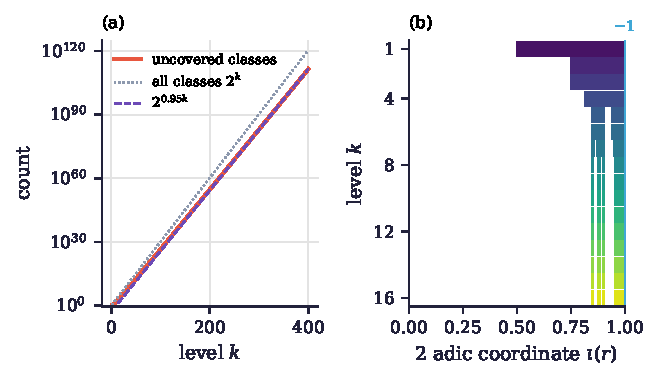
\includegraphics[width=\textwidth]{figures/ch10b_sieve.pdf}
\caption{The residue sieve. (a) The number of classes modulo $2^k$ not certified
to descend within $k$ steps, computed exactly up to $k=400$, against all $2^k$
classes and the growth rate $2^{0.95k}$. (b) The uncovered classes at levels
$1$ to $16$ drawn in the $2$ adic coordinate $\iota(r)=\sum r_i2^{-i-1}$; they
shrink to a closed set of measure zero that contains $-1$, the point at the
right edge, whose orbit never descends.}
\label{fig:ch10b:sieve}
\end{figure}

\Cref{thm:ch5c:residue} gives the same conclusion from the side of
optimization: the residue graph has cycles of positive mean weight, so no potential $\log x+\varphi(x\bmod2^k)$ with bounded $\varphi$ decreases at every step for all large $x$.
The structural reason is $2$ adic. Let $E\subset\Z_2$ be the set of $2$ adic
integers whose parity sequence under $T$ satisfies $3^{m_j}>2^j$ for every $j$,
the points with infinite coefficient stopping time.

\begin{proposition}[What residue certificates can and cannot do]
\label{prop:ch10b:residue}
\leavevmode
\begin{enumerate}[label=(\roman*),leftmargin=2em]
\item $E$ is a closed subset of $\Z_2$ of Haar measure zero, it is the
  intersection over $k$ of the unions of uncovered classes at level $k$, and it
  contains $-1$, $-5$ and $-17$, one point of each of the three known cycles of $T$ on the negative
  integers.
\item Every uncovered class at every level contains infinitely many positive
  integers. Hence no residue certificate of finite level covers all integers
  $n\ge2$.
\item If a positive integer $n\ge2$ lies in $E$, its orbit never falls below
  $n$. Hence the descent form of the conjecture implies $E\cap\{2,3,\ldots\}=
  \emptyset$, and conversely this together with the coefficient stopping time
  conjecture of \cref{chap:parity} implies the descent form.
\end{enumerate}
\end{proposition}

\begin{proof}
(i) The uncovered set at level $k$, $E_k$, is a finite union of balls
$r+2^k\Z_2$, hence closed, and $E=\bigcap_kE_k$ because the parity vector of a
$2$ adic integer of length $k$ depends only on its class modulo $2^k$. Its
measure is $\lim_k(1-F(k))=0$ by \cref{thm:density}. The point $-1$ is fixed by
$T$ and odd, so $m_j=j$ and $3^j>2^j$ for all $j$. For a point of a negative cycle with $r$ odd steps in a period of $s$ steps,
$3^r>2^s$ by the reversed cycle identity\index{cycle identity} of \cref{chap:cycles}, so the ratio
$3^{m_j}/2^j$ is multiplied by $3^r/2^s>1$ over each period; hence it exceeds $1$
for every $j$ as soon as it does for $j\le s$, and a direct check over one period
confirms this for $-5$ (period $3$) and $-17$ (period $11$), though not for the
other points of those cycles. (ii) A class $r+2^k\Z$ contains
$r+2^kt$ for every $t\ge1$. (iii) If $n\in E$ then
$T^{(j)}(n)=(3^{m_j}n+c_j)/2^j>n$ for every $j$, since $c_j\ge0$. The converse uses
the conjecture of Terras that the coefficient stopping time equals the stopping
time for every $n\ge2$.
\end{proof}

The proposition isolates exactly what computation on residues can deliver: the descent form of the conjecture implies that no integer $n\ge2$ lies in the measure zero closed set $E$, and the converse holds if the coefficient stopping time conjecture of Terras\index{Terras, R.} holds (\cref{rem:ch2:cst}).
Positive integers are the
$2$ adic integers whose digits are eventually all $0$, while the known points of
$E$, such as $-1=\ldots1111$, have digits eventually all $1$ or eventually
periodic. The remaining statement is an integrality property, a statement about
how $E$ meets the eventually zero sequences, and no finite residue computation
can establish it, because every finite level leaves balls of $E_k$ that contain
both integers and points of $E$.

\section{Automated termination provers}\label{sec:ch10b:automated}

The most ambitious computational attack to date takes the certificate\index{certificate} idea to its
logical end. Yolcu\index{Yolcu, E.}, Aaronson\index{Aaronson, S.} and Heule\index{Heule, M. J. H.}~\cite{yolcu2023} encode the Collatz map as a
string rewriting\index{rewriting system} system acting on mixed binary and ternary representations,
prove that termination of the system is equivalent to the conjecture, and search
for termination proofs by matrix interpretations, a standard technique in which
each rewriting rule must decrease a weight computed by multiplying small
matrices. Their prover found automatic proofs of nontrivial weakenings of the
conjecture, but not of the conjecture itself.

In the language of this book a matrix interpretation is a Lyapunov function\index{Lyapunov function} of
a special kind: the weight of a word is a linear function of a product of
matrices indexed by its letters, so it is a potential that reads the digits of
$n$ through a finite automaton. \Cref{prop:ch10b:residue} explains why such
potentials face the same obstruction as residue certificates\index{residue sieve} when they read
only boundedly many digits, and why the mixed representation matters: a
ternary digit records information about $n$ that its binary residues do not, so
an automaton reading both can in principle see the integrality that separates
the positive integers from $E$. That is the most promising feature of the
approach, and the reason it is a natural place for the large scale computation
of a coming decade.

\section{Does the MM view offer guidance?}\label{sec:ch10b:guidance}

It does, in several specific ways.

\paragraph{The potential.} The martingale duality of \cref{chap:stochastic}
constrains the potential: in the Bernoulli model for $T$, $x_n$ itself has no drift\index{drift}, $\log x_n$ has drift
$\log(\sqrt3/2)$, and $x_n^\theta$ decreases in expectation exactly when $0<\theta<1$ (\cref{thm:martingale}).
Any certificate\index{certificate} whose leading term grows at least linearly in $n$, such as one built on $n$ or on $n^\theta$ with $\theta\ge1$, fights the martingale\index{martingale}, which is why linear majorizer\index{majorization}s fail (\cref{prop:mmfails}); the powers $n^\theta$ with $0<\theta<1$ decrease in expectation but, like $\log n$, only on average over residue classes.
Matrix interpretations
measure size multiplicatively, through products, which is the right
geometry.

\paragraph{The horizon.} \Cref{thm:nolyapunov,cor:ch4:multistride} and the comments after them show that no monotone certificate with a fixed horizon exists: for every $J$ there are integers whose first $J$ strides all ascend, which defeats every nondecreasing potential, and $S^{(J)}(5)=1$ for every $J\ge1$, which defeats every nonincreasing one. An MM certificate built on a monotone potential such as $\log x$ must
therefore majorize over a \emph{variable} horizon, the number of steps to the
first descent, which is the stopping time\index{stopping time}. The greedy scheme ``iterate until
the potential has decreased, then majorize afresh'' is exactly the stopping time
decomposition of \cref{chap:parity}, and the conjecture in descent form is the
statement that this greedy MM is well defined at every $n\ge2$. The MM language
thus turns the conjecture into a termination statement for a specific
algorithm, which is precisely the form a termination prover needs.

\paragraph{The switching.} For Switching MM the joint spectral radius of the two modes, computed exactly by \cref{prop:ch5b:jsr}, is below one at every parameter value computed, and at all values if \cref{conj:ch5b:transient} holds; every switching sequence is then safe (\cref{cor:ch5b:anyswitch}).
For the Collatz switched system\index{switched system}
\eqref{eq:ch5b:switched} the opposite holds: some switching sequences diverge, the all odd one for instance, and
by the theorem of Terras\index{Terras, R.} and Everett\index{Everett, C. J.} (\cref{thm:terras}) every parity word of every length is realized by a residue
class containing arbitrarily large integers. So there is no constraint on the
switching signal at any finite horizon, and the constrained switching methods
of control theory, which certify stability by restricting the admissible
switching sequences to the language of a finite automaton, have nothing to work
with. Whatever constrains the Collatz signal couples the parity sequence to the
size and the digits of the state. This is the switched systems form of
\cref{prop:ch10b:residue}.

\paragraph{The potential, pressed.} \Cref{chap:mmcollatz} pushes the
majorization idea to its limit and proves three impossibility results for potentials that decrease at every step: no potential $\log x+\varphi(x\bmod2^k)$ with bounded $\varphi$ decreases at every step for all large $x$, for any $k$, because the cycles of
$T$ on the negative integers\index{negative cycles} are positive cycles of every residue graph
(\cref{thm:ch5c:residue}); any pointwise potential that decreases at every stride must give integers with $j$
trailing ones a surplus growing like $j\log(3/2)$ (\cref{prop:ch5c:surplus});
and the block potentials that supply this surplus fail, in the model, at a fraction of odd
integers that no weight brings below $0.143$ (\cref{prop:ch5c:runpot}). The
same chapter shows that the cycle inequality is the bound of the multiplicative
majorizer\index{MM algorithm} summed around the cycle, so for the cycle half majorization is a
reformulation and not a method.

\paragraph{The memory.} Accelerated methods need Lyapunov functions of two
consecutive iterates (\cref{sec:ch5b:stability}), and one might hope that a
potential with memory, depending on the recent history of the orbit, could
certify Collatz descent.
A memory of bounded length, however, adds only boundedly many parities, since $x_{n-1}$ is determined by $x_n$ and the parity of $x_{n-1}$, and a potential $\log x_n+\varphi$ with $\varphi$ bounded, whatever part of that history and of the residues of $x_n$ it reads, still increases along the long runs of odd steps from integers $2$ adically close to $-1$, as in \cref{thm:ch5c:residue}.
Memory helps only if it records unbounded
arithmetic information, the digits that decide integrality.

\paragraph{Polyak.} A reader of \cref{chap:momentum,chap:difference} may ask
whether Polyak\index{Polyak, B. T.}'s results, which underlie the momentum method, have anything
to offer here. Four of them are relevant and none of them transfers. The heavy
ball method\index{heavy ball}~\cite{polyak1964} is what Switching MM specializes, and its analysis is exactly
the switched system of \cref{chap:difference}; it tells us how the Collatz
schedule behaves as an optimizer, not how the integers behave. The gradient
dominance, or Polyak and \L{}ojasiewicz\index{Lojasiewicz, S.@\L{}ojasiewicz, S.}, inequality\index{Polyak and Lojasiewicz@Polyak and \L{}ojasiewicz inequality}
$\|\nabla f\|^2\ge2\mu(f-f^\ast)$~\cite{polyak1987} is the condition that makes linear rates
possible without convexity, and it is a pointwise condition: it would require
$\log x$ to decrease at every step by a fixed fraction of its distance to the
minimum, which the ascents of \cref{thm:nolyapunov} rule out. The Collatz
drift is additive and holds only in expectation, which is Foster\index{Foster, F. G.}'s condition
for Markov chains, not Polyak's for descent methods. Polyak and Ruppert\index{Ruppert, D.}
averaging~\cite{ruppert1988,polyak1990,polyak1992}, the device by which a noisy iteration achieves the optimal rate by
averaging its iterates, corresponds under the logarithm to the Ces\`aro
criterion of \cref{chap:divergence}: it is the right object to look at and it
is the statement that remains unproved. Finally the Polyak step size
$\alpha_k=(f(x_k)-f^\ast)/\|\nabla f(x_k)\|^2$~\cite{polyak1987} needs the optimal value, which
for Collatz is $f^\ast=\log1=0$ and is known; but the Collatz step sizes are
not ours to choose, the parity sequence chooses them, and a method that
adapts its step to the distance from the optimum has nothing to adapt.
Polyak's results are therefore useful for the optimizer in Part II and
irrelevant to the conjecture in Part III, which is the same division the rest
of the book makes.

So the optimization reading does not shorten the path, but it marks it. It says
which potentials can work, that the horizon of a monotone certificate must be variable, that parity
information of bounded length can never suffice, and that the missing ingredient is an
integrality argument, a way of using the fact that $n$ has a terminating binary
expansion. These are also features of the most serious computational
programme now in existence.

\section*{Notes}

The $2$ adic formulation of the stopping time\index{stopping time} problem is due to Terras\index{Terras, R.} and to
Lagarias\index{Lagarias, J. C.}~\cite{lagarias1985}, and Bernstein\index{Bernstein, D. J.}~\cite{bernstein1994} gives a
noniterative form. The rewriting\index{rewriting system} approach and the matrix interpretation prover
are from Yolcu\index{Yolcu, E.}, Aaronson\index{Aaronson, S.} and Heule\index{Heule, M. J. H.}~\cite{yolcu2023}.
The residue sieve\index{residue sieve} counts to $k=400$ and the divisibility sieve experiment are ours.
The exponent $h=H(1/\lt)$ gives the decay rate $1-h$ of Lagarias\index{Lagarias, J. C.}'s exponential form of the density theorem of Terras\index{Terras, R.} and Everett\index{Everett, C. J.}, $1-F(k)\le2^{-(1-h)k}$~\cite[Theorem~D]{lagarias1985}.
\Cref{prop:ch10b:residue} in the form stated is ours, although each ingredient of the proposition is classical.

\section*{Exercises}

\begin{exercise}
Using the recursion of \cref{prop:ch2:dp}, show that the number of uncovered
classes modulo $2^k$ is equal to the number of binary words of length $k$ all of
whose prefixes have a proportion of ones above $1/\lt$, and deduce that it grows
like $2^{(h+o(1))k}$ with $h=H(1/\lt)$ (the binomial tail gives the upper bound).
\end{exercise}

\begin{exercise}
Run the divisibility sieve of \cref{sec:ch10b:cycles} for $(m,k)=(8,13)$ by
hand or by machine, find the residues of $c_{13}(w)$ modulo $233$ that occur, and
confirm that $0$ is not among them. How many words are there, and how does that
compare with $233$?
\end{exercise}

\begin{exercise}
Show that the rational number $1/5$ is periodic under the accelerated map\index{accelerated map} on
$\Z_2$ with odd denominators allowed, and decide whether it lies in $E$.
\end{exercise}

\begin{exercise}
Explain why a potential $V(n)=\log n+\varphi(n\bmod2^k)$ with $\varphi$ bounded
cannot certify descent over a fixed horizon $J$ for all $n\ge2$, by exhibiting
integers in the class $-1\bmod2^{J+1}$ for which $V$ increases over $J$ steps
once $n$ is large.
\end{exercise}
